\renewcommand{\NomeBloco}{\textit{APS\_3}}
\renewcommand{\NomeBlocoNoUnderline}{apsthree}
\renewcommand{\NomePTab}{tab_\NomeBlocoNoUnderline}
\renewcommand{\NomeSTab}{tab_\NomeBlocoNoUnderline2}
\renewcommand{\NomePFig}{fig_\NomeBlocoNoUnderline}
\renewcommand{\NomeSFig}{fig_\NomeBlocoNoUnderline2}
\renewcommand{\NomeTTab}{tab_\NomeBlocoNoUnderline3}
\renewcommand{\NomeQTab}{tab_\NomeBlocoNoUnderline4}

\section{APS\_3}

O \textit{\NomeBloco} \'e o circuito respons\'avel por armazenar todos os tr\^es blocos APS de cor (Azul, Verde, Vermelho), mais o TIA geradora de rel\'ogio de refer\^encia para os APS's citados. O bloco apresenta as definicões de sa\'ida referidos na \autoref{\NomeSTab}.

As sa\'idas digitais de cada bloco APS\_3 apresentam um buffer, de forma a garantir a integridade do sinal nos pinos do Circuito Integrado.

\begin{figure}[!h]
 \centering
    \centering
    \caption{\label{\NomeSFig}Representacão em bloco do \NomeBloco}
    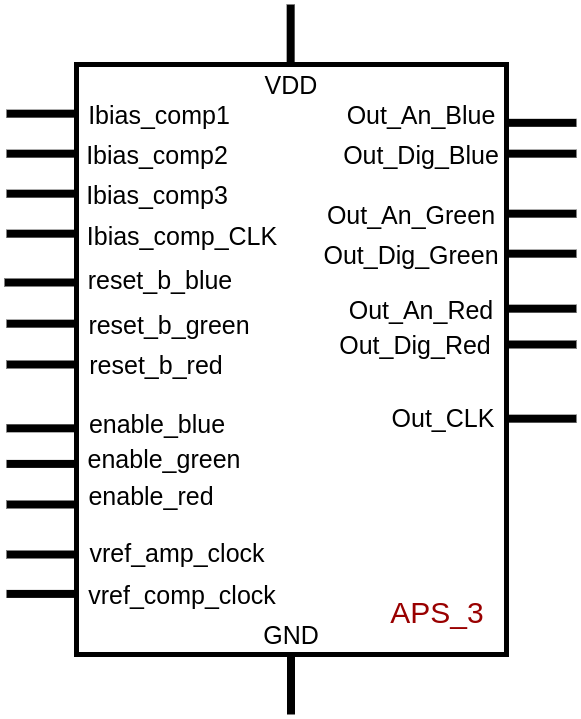
\includegraphics[scale=0.3]{Circuitos/APS_3_block.png}
    \legend{Fonte: Produzido pelo autor}
\end{figure}

\begin{table}[!h]
\centering
  \caption{Descricão dos sinais de entrada e sa\'ida do circuito projetado para as cores azul, verde e vermelha}%
  \label{\NomeSTab}
  \begin{tabular}{ccll}
  \toprule
   Sinal & Tipo & Descricão & Observacão \\
  \midrule \midrule
   RESET\_BLUE & Entrada & \begin{tabular}[l]{@{}l@{}}Sinal de tensão \textit{RESET}\\ no APS para cor azul\end{tabular} & Ativo em n\'ivel baixo \\
  \midrule
   RESET\_GREEN & Entrada & \begin{tabular}[l]{@{}l@{}}Sinal de tensão de \textit{RESET}\\ no APS para cor verde\end{tabular} & Ativo em n\'ivel baixo \\
  \midrule
   RESET\_RED & Entrada & \begin{tabular}[l]{@{}l@{}}Sinal de tensão \textit{RESET}\\ no APS para cor vermelha\end{tabular} & Ativo em n\'ivel baixo \\
   \midrule
   ENABLE\_BLUE & Entrada & \begin{tabular}[l]{@{}l@{}}Sinal de tensão \textit{ENABLE} \\no APS para cor azul\end{tabular} & Ativo em n\'ivel alto \\
  \midrule
   ENABLE\_GREEN & Entrada & \begin{tabular}[l]{@{}l@{}}Sinal de tensão \textit{ENABLE} \\no APS para cor verde\end{tabular} & Ativo em n\'ivel alto \\
  \midrule
   ENABLE\_RED & Entrada & \begin{tabular}[l]{@{}l@{}}Sinal de tensão \textit{ENABLE}\\ no APS para cor vermelha\end{tabular} & Ativo em n\'ivel alto \\
  \midrule
   Ibias\_comp1 & Entrada & \begin{tabular}[l]{@{}l@{}}Fonte de corrente para\\ cor Azul\end{tabular} &  \\
   \midrule
   Ibias\_comp2 & Entrada & \begin{tabular}[l]{@{}l@{}}Fonte de corrente para\\ cor Verde\end{tabular} &  \\
   \midrule
   Ibias\_comp3 & Entrada & \begin{tabular}[l]{@{}l@{}}Fonte de corrente para\\ cor Vermelha\end{tabular} &  \\
   \midrule
   Ibias\_clk & Entrada & \begin{tabular}[l]{@{}l@{}}Fonte de corrente para o\\ bloco \textit{APS\_pixel\_clk}\end{tabular}
    &  \\
  \midrule
   Out\_An\_Blue & Sa\'ida & \begin{tabular}[l]{@{}l@{}}Sinal anal\'ogico para cor\\ azul\end{tabular} \\
  \midrule
   Out\_Dig\_Blue & Sa\'ida & Sinal digital para cor azul \\
  \midrule
   Out\_An\_Green & Sa\'ida & \begin{tabular}[l]{@{}l@{}}Sinal anal\'ogico para cor\\ verde\end{tabular} \\
  \midrule
   Out\_Dig\_Green & Sa\'ida & Sinal digital para cor verde \\
  \midrule
   Out\_An\_Red & Sa\'ida & \begin{tabular}[l]{@{}l@{}}Sinal anal\'ogico para cor\\ vermelha\end{tabular} \\
  \midrule
   Out\_Dig\_Red & Sa\'ida & \begin{tabular}[l]{@{}l@{}}Sinal digital para cor\\ vermelha\end{tabular} \\
  \bottomrule
  \end{tabular}
  \legend{Fonte: Produzido pelo autor.}
\end{table}

O circuito projetado para o bloco \'e demonstrado na \autoref{\NomePFig}.

\clearpage

\begin{figure}[!h]
 \centering
    \centering
    \caption{Circuito CMOS projetado para o bloco \NomeBloco} 
    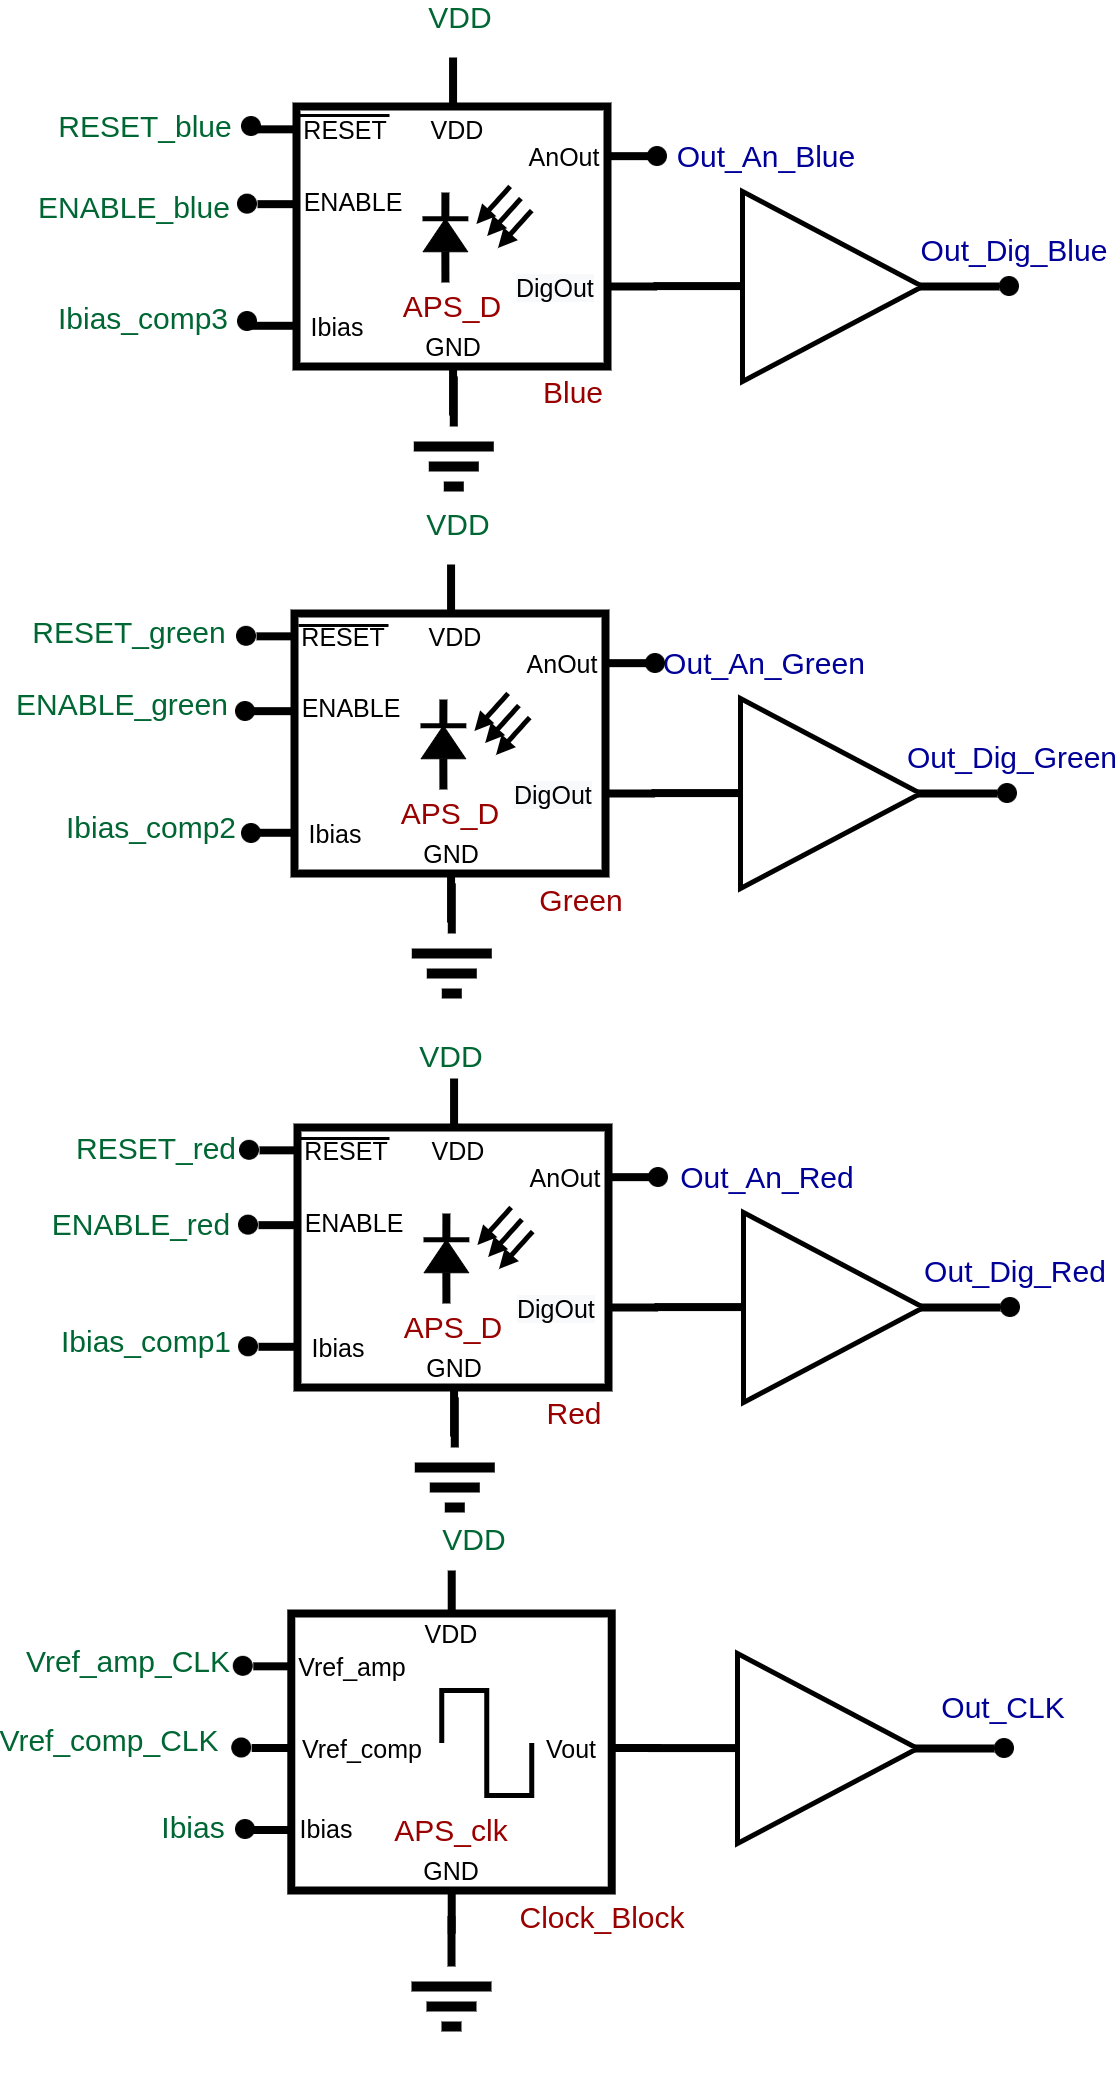
\includegraphics[scale=0.3]{Circuitos/APS_3.png}
    \legend{Fonte: Produzido pelo autor}
    \label{\NomePFig}
\end{figure}